\thispagestyle{empty}
\section{Решения контрольной номер 3. ИП}




\subsection[2018-2019]{\hyperref[sec:kr_03_ip_2018_2019]{2018-2019}}
\label{sec:sol_kr_03_ip_2018_2019}

\begin{enumerate}
\item
\begin{enumerate}
\item Пары ортогональных величин: $(X_1,X_2); (X_2,X_3); (X_1,X_3); (S_2,X_3)$.
\item В качестве примера можно взять величину $X_2-X_1$, поскольку
\begin{align*}
\Cov(X_2-X_1,S_3) &= \Cov(X_2-X_1,X_1+X_2+X_3) \\
&= \Var(X_1)-\Var(X_1)=0
\end{align*}
\item Как известно из линейной алгебры, если вектор $X^-_1$ — проекция $X_1$ на $S_3$,
a $X^{\perp}_1$ — соответствующая ортогональная составляющая, то $X^{\perp}_1=X_1-X^-_1 = X_1-\alpha S_3$,
причем
\[
\langle X^{\perp}_1,S_3\rangle = \Cov(X^{\perp}_1,S_3) = \Cov(X^{\perp}_1,X_1-\alpha S_3) = 0,
\]
откуда
\[
\alpha = \frac{\Cov(X_1,S_3)}{\Var(S_3)}.
\]
Тогда искомая проекция равна
\[
\frac{\Cov(X_1,S_3)}{S_3}\cdot S_3
\]
\item Искомая проекция равна ортогональной составляющей из предыдущего пункта:
\[
X^{\perp}_1 = X_1 - \frac{\Cov(X_1,S_3)}{S_3}\cdot S_3
\]
\item Пусть соответствующие проекции равны $X^-_1 = \alpha S_3$, $X^-_2 = \beta S_3$.
Тогда
\begin{align*}
\Cov(X^-_1,X^-_2) &= \Cov(X_1-\alpha S_3,X_2 - \beta S_3) \\
&=-\alpha\Var(X_1)-\beta\Var(X_2)+3\alpha\beta\Var(X_1)
\end{align*}
\begin{align*}
\Var(X^-_1) &= \Var(X_1 - \alpha S_3)\\
&= \Var(X_1) + 3\alpha^2\Var(X_1) - 2\alpha\Var(X_1)
\end{align*}

Заметим, что дисперсии величин $X_1$ и $X_2$ равны, поэтому
\begin{align*}
\Var(X^-_2) &= \Var(X_2 - \beta S_3)\\
&= \Var(X_1) + 3\beta^2 \Var(X_1) - 2\beta\Var(X_1)
\end{align*}

Таким образом, искомая частная корреляция равна
\[
\frac{(3\alpha\beta - \alpha - \beta)\Var(X_1)}{\Var(X_1)\sqrt{(1 - 2\alpha + 3\alpha^2)(1 - 2\beta + 3\beta^2)}}
\]

Вспоминаем, что
\[
\alpha = \frac{\Cov(X_1,S_3)}{\Var(S_3)} = \frac{\Var(X_1)}{3\Var(X_1)} = \frac{1}{3} = \beta,
\]
откуда искомая частная корреляция равна $-1/2$.
\end{enumerate}
\item
\begin{enumerate}
\item Как видно по графику, $x-1\geq \ln x$.
\begin{figure}[ht!]
\begin{center}
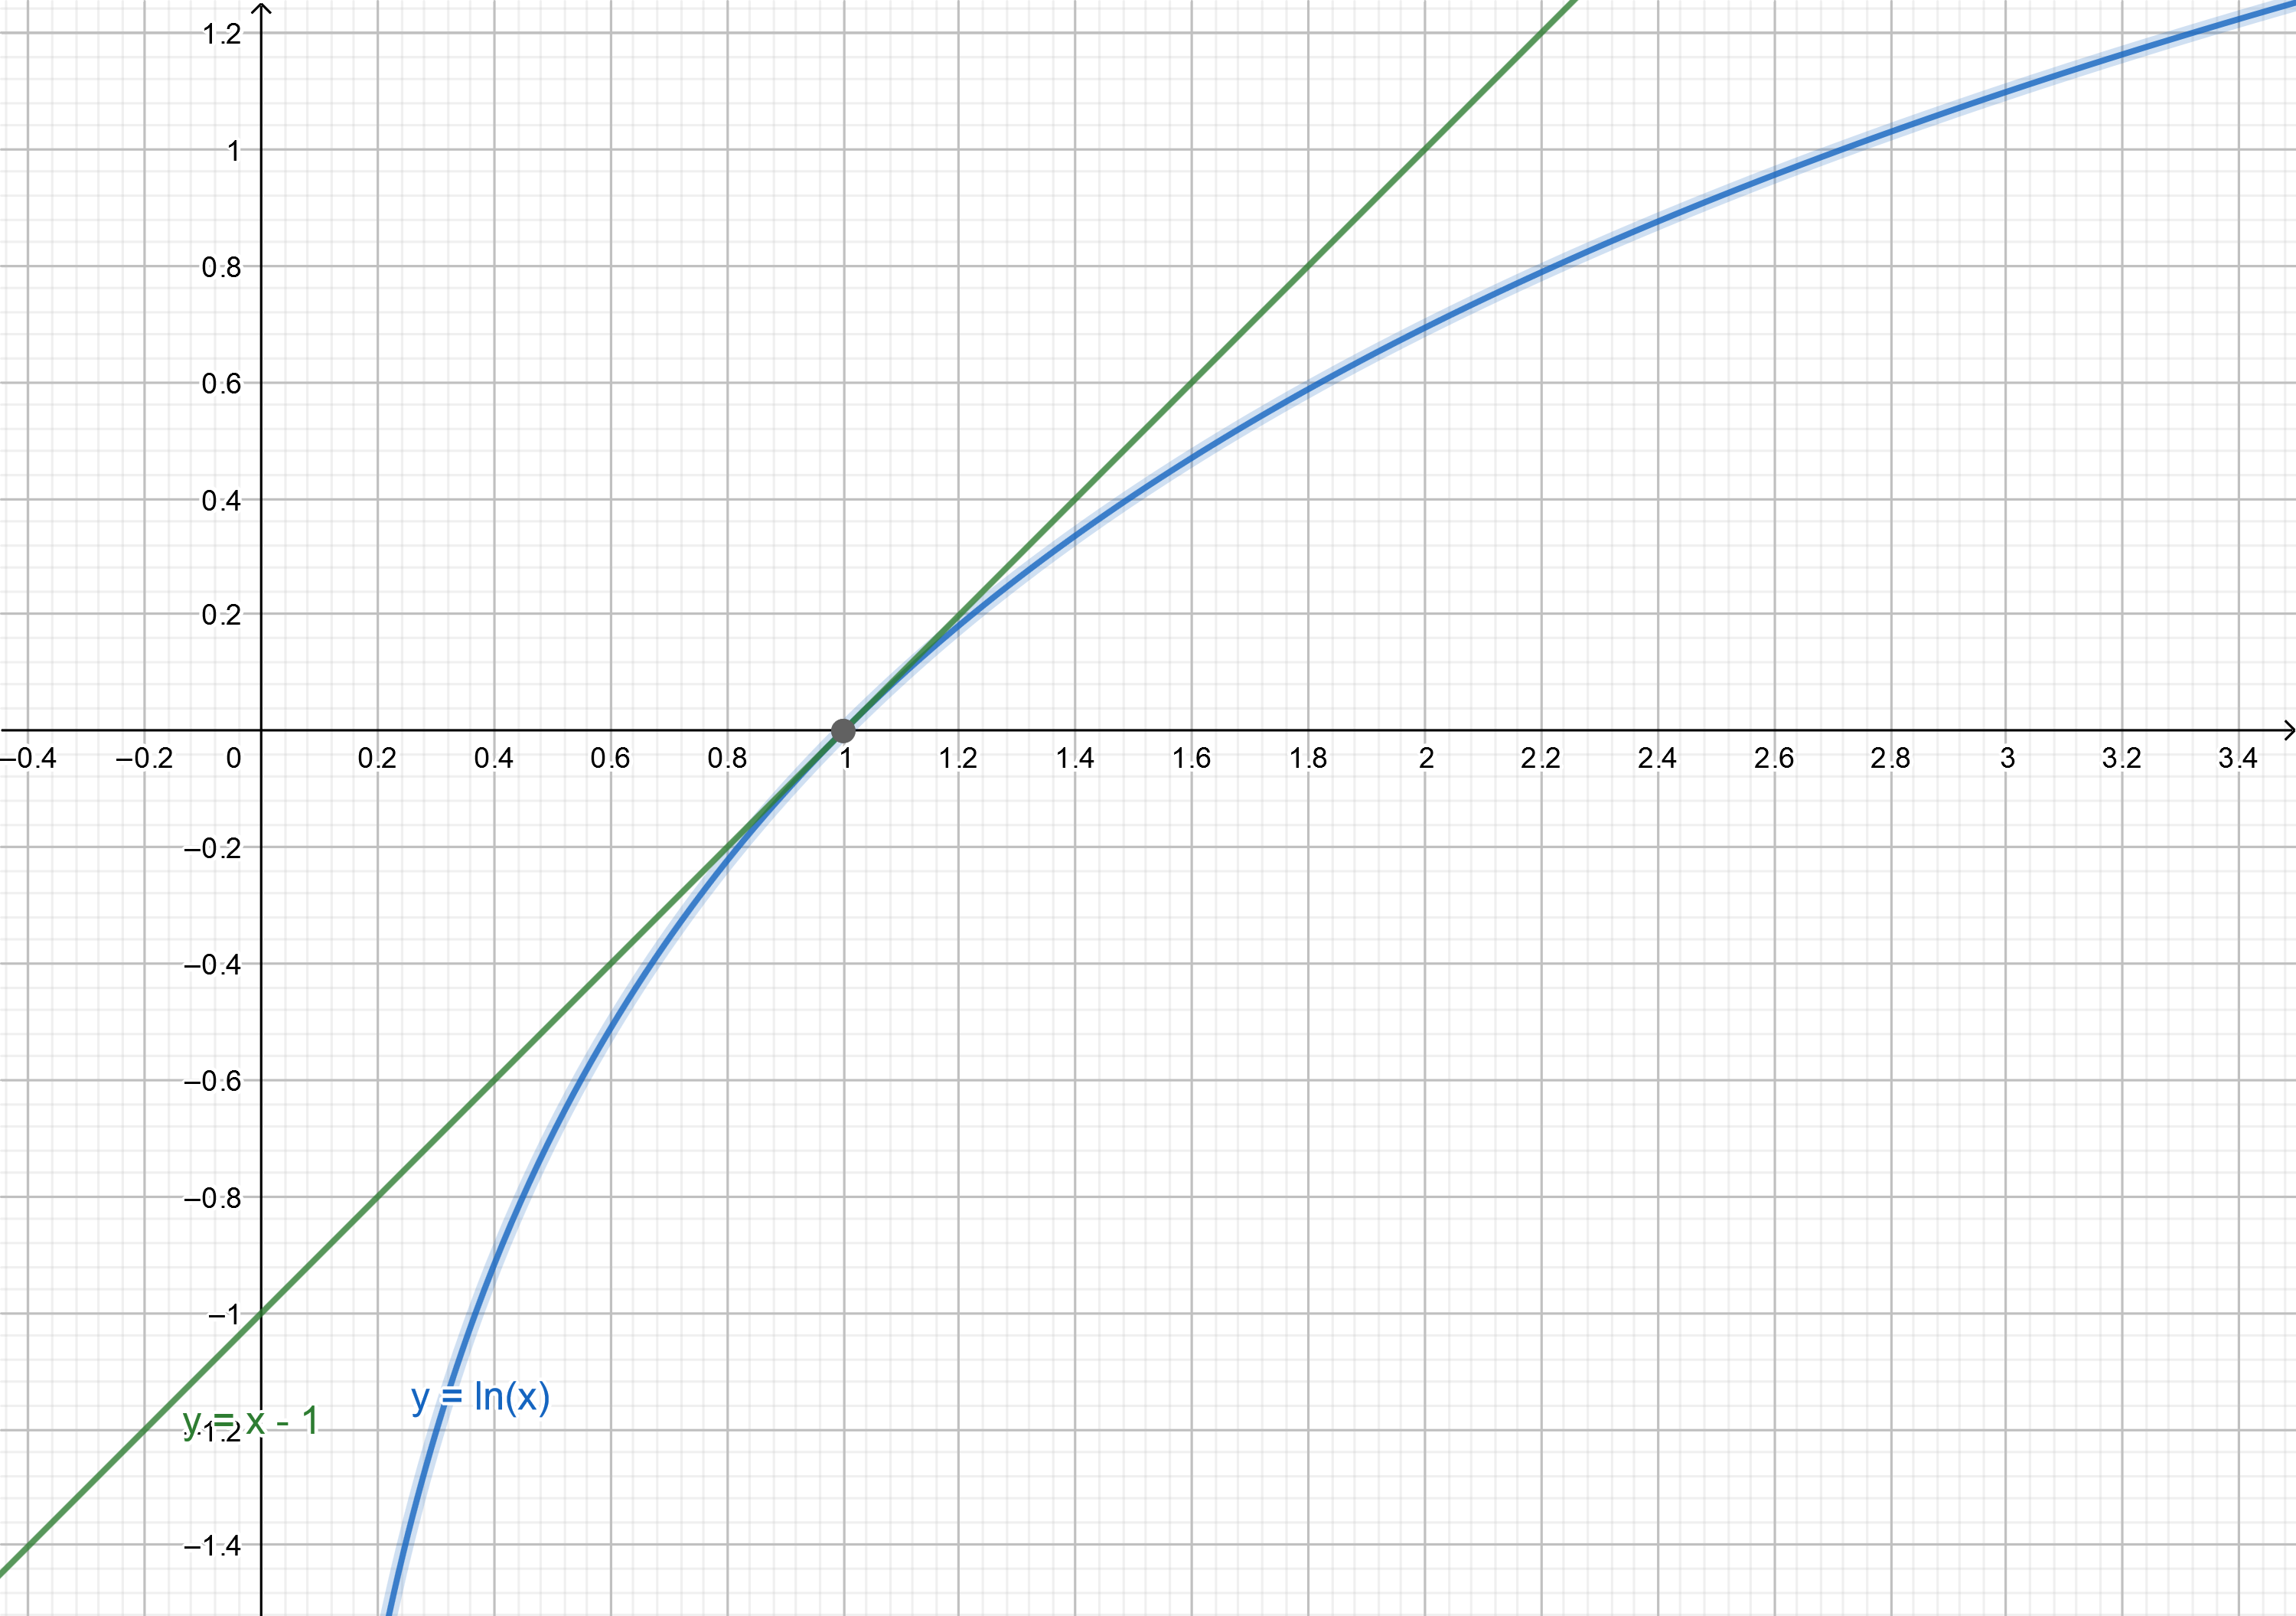
\includegraphics[]{images/sol_kr_3_ip.png}
\end{center}
\end{figure}
\item По свойству из предыдущего пункта,
\begin{align*}
\frac{q(x)}{p(x)} - 1 &\geq \ln \left(\frac{q(x)}{p(x)}\right) \\
g(x)-p(x) &\geq p(x)\ln q(x)-p(x)\ln p(x) \\
-p(x)\ln q(x) & \geq -p(x)\ln p(x) + p(x) - q(x)
\end{align*}
Интегрируем:
\begin{align*}
-\int^{+\infty}_{-\infty}p(x)\ln q(x) \; dx \geq &-\int^{+\infty}_{-\infty}p(x)\ln p(x) \; dx \\
&+\int^{+\infty}_{-\infty}p(x) \; dx - \int^{+\infty}_{-\infty}q(x) \; dx
\end{align*}
Поскольку $p(x)$, $q(x)$ – функции плотности, интегрирование каждой из них дает
единицу, а значит, последние два слагаемых в сумме равны нулю:
\[
-\int^{+\infty}_{-\infty}p(x)\ln q(x) \; dx \geq -\int^{+\infty}_{-\infty}p(x)\ln p(x) \; dx
\]
\item Функция плотности для величины $X \sim \cN(\mu;\sigma^2)$ есть
\begin{align*}
q(x)&=\frac{1}{\sqrt{2\pi\sigma^2}}\exp{\left(\frac{-(x-\mu)^2}{2\sigma^2}\right)}\\
\ln q(x)&=-\frac{1}{2}\ln 2\pi-\ln \sigma-\frac{(x-\mu)^2}{2\sigma^2}\\
H(q)&=-\int^{+\infty}_{-\infty}q(x)\ln q(x) \; dx
\end{align*}
\begin{align*}
H(q)&=\int^{+\infty}_{-\infty}q(x)\left(\frac{1}{2}\ln 2\pi+\ln \sigma+\frac{(x-\mu)^2}{2\sigma^2}\right) \; dx\\
&=\frac{1}{2}\ln 2\pi + \ln \sigma+\int^{+\infty}_{-\infty}q(x)\frac{(x-\mu)^2}{2\sigma^2} \; dx\\
&=\frac{1}{2}\ln 2\pi + \ln \sigma+\int^{+\infty}_{-\infty}\frac{\left(q(x)x^2-2x\mu q(x)+\mu^2q(x)\right)}{2\sigma^2} \; dx\\
&=\frac{1}{2}\ln 2\pi + \ln \sigma+\frac{1}{2\sigma^2}\left(\E(X^2)-2\mu\E(X)+\mu^2\right)\\
&=\frac{1}{2}\ln 2\pi + \ln \sigma+\frac{1}{2\sigma^2}\left(\sigma^2+\mu^2-2\mu^2+\mu^2\right)\\
&=\frac{1}{2}\ln 2\pi + \ln \sigma+\frac{1}{2}
\end{align*}
\item Пусть $Y \sim \cN(\mu_N;\sigma^2_N)$, ее функция плотности равна $q(x)$. Тогда, аналогично пункту в), получаем:
\begin{align*}
CE_p(q) &= \frac{1}{2}\ln 2\pi + \ln \sigma_N +\int^{+\infty}_{-\infty}\frac{\left(p(x)x^2-2x\mu_N p(x) + \mu^2_Np(x)\right)}{2\sigma^2_N} \; dx\\
&= \frac{1}{2}\ln 2\pi + \ln \sigma_N + \frac{1}{2\sigma^2_N}\left(\sigma^2 + \mu^2-2\mu\mu_N + \mu^2_N\right)
\end{align*}
\end{enumerate}
\item
\begin{enumerate}
\item[a)]
\begin{align*}
L&=\lambda e^{-\lambda x_1}\lambda e^{-\lambda x_2}\\
\ln L&=2\ln \lambda-\lambda(x_1+x_2)\\
(\ln L)'_\lambda&=\frac{2}{\hat{\lambda}}-(x_1+x_2)=0\\
\hat{\lambda}&=\frac{2}{x_1+x_2}=\frac{1}{15}
\end{align*}
\item[б)] Пусть $X$ – время обслуживания одного клиента, тогда
\begin{align*}
\P(X>30)&=\int^{+\infty}_{30}\lambda e^{-\lambda x} \; dx \Rightarrow\\
L&=\lambda e^{-\lambda x_1}\lambda e^{-\lambda x_2}\prod^{10}_{i=3}\int^{+\infty}_{30}\lambda e^{-\lambda x_i} \; dx_i\\
\int^{+\infty}_{30}\lambda e^{-\lambda x} \; dx&=-e^{-\lambda x}|^{+\infty}_{30}=e^{-30\lambda}\\
L&=\lambda e^{-\lambda x_1}\lambda e^{-\lambda x_2}\prod^{10}_{i=3}e^{-30\lambda}\\
\ln L&=2\ln \lambda-\lambda(x_1+x_2)-240\lambda\\
(\ln L)'_\lambda&=\frac{2}{\hat{\lambda}}-(x_1+x_2)-240=0\\
\hat{\lambda}&=\frac{1}{135}
\end{align*}
\item
\begin{align*}
\P(X<30)&=1-\int^{+\infty}_{30}\lambda e^{-\lambda x} \; dx=1-e^{-30\lambda} \Rightarrow\\
L&=\prod^{2}_{i=1}(1-e^{-30\lambda})\prod^{10}_{i=3}e^{-30\lambda}\\
\ln L&=2\ln (1-e^{-30\lambda})-240\lambda\\
(\ln L)'_\lambda&=\frac{2\cdot30e^{-30\hat{\lambda}}}{1-e^{-30\hat{\lambda}}}-240=0\\
\hat{\lambda}&\approx0,0074
\end{align*}
\item[г)]
\begin{align*}
L&=\lambda e^{-\lambda x_1}\lambda e^{-\lambda x_2}\prod^{10}_{i=3}e^{-20\lambda}\\
\ln L&=2\ln \lambda-\lambda(x_1+x_2)-160\lambda\\
\hat{\lambda}&=\frac{1}{95}
\end{align*}
\end{enumerate}
\item У всех одинаковые нулевые шансы стать Самым Главным, 
что можно доказать методом математической индукции. 
Пусть всего метеорологов двое. Тогда, если у них монеты
упали одной стороной, они оба выбывают, если разными, то игра продолжается. 
Если метеорологов трое и у всех монеты выпали одной стороной, то все выходят из игры;
если у одного из них выпала решка, а у остальных – орлы, то первый выбывает, 
получаем ситуацию для двух и так далее.
\item
\begin{enumerate}
\item Обозначим количества орлов в соответствующие дни за $S_1$, $S_2$, $S_3$,
а количества бросков – за $n_1$, $n_2$, $n_3$. По своим данным Анна может построить
оценку $\hat{p}_a=(S_1+S_2)/(n_1+n_2)$, а Белла – $\hat{p}_b=(S_2+S_3)/(n_2+n_3)$.
Наша цель – минимизировать по $\alpha$ дисперсию взвешенной оценки:
\[\Var(\hat{p})=\Var(\alpha\hat{p}_a+(1-\alpha)\hat{p}_b)\]
Или явно:
\begin{align*}
    p(1 - p)\left(\frac{\alpha}{n_1 + n_2} + \frac{(1 - \alpha)^2}{n_2 + n_3} +
    \frac{2\alpha(1 - \alpha)n_2}{(n_1 + n_2)(n_2 + n_3)}\right)
\end{align*}
\[
\alpha^*=\frac{n_1}{n_1+n_3}
\]
Оценки: $\hat{p}_a=0.4$, $\hat{p}_b=0.5$, $\alpha=0.4$, $\hat{p}=0.46$.

\item Подставим найденную $\alpha^*$ в формулу для дисперсии и получим
\[
\frac{n_1n_2+n_2n_3+n_1n_3}{(n_1+n_2)(n_1+n_3)(n_2+n_3)}p(1-p)
\]
При наших данных $\hat{\Var}(\hat{p})\approx0.0458$.

\item Используя стандартную формулу, получим:
\[
[\hat{p}-1.96se(\hat{p});\hat{p}+1.96se(\hat{p})],
\]
где $\hat{p}=0.46$ и $se(\hat{p})\approx0.214$.
\end{enumerate}
\end{enumerate}


\subsection[2017-2018]{\hyperref[sec:kr_03_ip_2017_2018]{2017-2018}}
\label{sec:sol_kr_03_ip_2017_2018}

\begin{enumerate}
\item
\begin{enumerate}
	\item[а) - в)] См. картинку :)
\begin{figure}[h!]
\centering
\begin{tikzpicture}
\coordinate (e) at (1,0);
\coordinate (X) at (4,3);
\coordinate (hatX) at (4,0);
\coordinate (perpX) at (0,3);
\draw[->] (0,0) -- (e);
\node [below] at (e) {e};
\draw[->] (0,0) -- (X);
\node [right] at (X) {X};
\draw[->] (0,0) -- (hatX);
\node [below] at (hatX) {$\hat{X}$};
\draw[->] (0,0) -- (perpX);
\node [left] at (perpX) {$\hat{X}^{\perp}$};
\draw [dashed] (perpX) -- (X);
\draw [dashed] (hatX) -- (X);
\end{tikzpicture}
\end{figure}
\item[г)] $\hat{X}=e\cdot\bar{X}$

$\lVert \hat{X} \rVert=\sqrt{n}\cdot\bar{X}$

$\hat{X}^{\perp}=X-e\cdot\bar{X}=(X_1-\bar{X}, \dots ,X_n-\bar{X})$

$\lVert\hat{X}^{\perp} \rVert =\sqrt{\sum^n_{i=1}(X_i-\bar{X})^2}$

\item[д)] $ \lVert X \rVert^2=\lVert\hat{X}^{\perp}\rVert^2+\lVert\hat{X}\rVert^2$

$\sum^n_{i=1}X^2_i=\sum^n_{i=1}(X_i-\bar{X})^2+n\bar{X}^2$

\item[е)] t-статистика для построения доверительного интервала для $\mu$ имеет вид:

\begin{align*}
t &= \frac{\bar{X}-\mu}{\sqrt{\bar{\sigma}^2/n}} = \frac{\bar{X}-\mu}{\sqrt{\sum^n_{i=1}(X_i-\bar{X})^2/(n\cdot(n-1))}}\\
& =\sqrt{n-1}\cdot\frac{\sqrt{n}\cdot(\bar{X}-\mu)}{\sqrt{\sum^n_{i=1}(X_i-\bar{X})^2}}=\sqrt{n-1}\cdot\frac{\lVert \hat{X} \rVert-\sqrt{n}\cdot\mu}{\lVert\hat{X}^{\perp} \rVert}
\end{align*}

Заметим, что $\ctg \alpha$ есть отношение прилежащего катета к противолежащему, таким образом, нужный нам угол $\alpha$ образуется между векторами $X$ и $\hat{X}$. Зметим однако, что в нашем случае
\[
t=\sqrt{n-1}\cdot \ctg \alpha=\frac{\lVert\hat{X}\rVert}{\lVert\hat{X}^{\perp}\rVert},
\]
то есть наша статистика подойдёт только для проверки гипотезе о равенстве матожидания нулю.

Замечание. $t=\sqrt{n-1}\cdot \ctg \alpha$ будет t-статистикой только в том случае, если $X_i$ будут н.о.р.с.в. с нормальным распределением, о чём в условие сказано не было.
\end{enumerate}
\item Выпишем функцию правдоподобия для выборки из трёх видов, два из которых совпадают. Первый медведепришелец будет нового вида с вероятностью 1. Вероятность, что вид второго пойманного медведепришельца совпадёт с первмым, составляет $1/n$. После этого нужно поймать медведепришельца нового вида – это произойдёт с вероятностью $(n-1)/n$, и ещё одного нового вида – вероятность этого $(n-2)/n$. Поскольку медведепришелец, вид которого встречается дважды, мог встретить на любой из трёх позиций, функцию правдоподобия необходимо домножить на $C_3^1$. Таким образом, функция правдоподобия имеет вид:
\[
L(n) = C_3^1 \cdot 1 \cdot \frac{1}{n} \cdot \frac{n-1}{n} \cdot \frac{n-2}{n}, n \geq 3.
\]
Максимизируя её, внутри области определения получаем $\hat n = 5$.

Так как количество медведей велико и все они встречаются равновероятно, то $p_{1}=p_{2}=p_{3}=1/n$. Так же из выборки известно, что число видов космомедведей не меньше трёх. Потому $\hat{n} \ge 3$.

Найдите хитрую ошибку в предложенном решении:

$L(n)=\left(\frac{1}{n}\right)^{2} \cdot \frac{1}{n}\cdot\frac{1}{n}=n^{-4}$

$\frac{\partial L(n)}{\partial n} = -4\cdot n^{-5}=0$

Данное уравнение не имеет решений при конечных $n$, но заметим, что при всех $n \ge 3$ выполняется $\frac{\partial L(n)}{\partial n} = -4\cdot n^{-5} < 0$, таким образом максимальное значение находится в граничных точках.

$\lim\limits_{n\to\infty}\frac{1}{n^{-4}}=0 < \frac{1}{3^{-4}}$

Таким образом получаем, что $\hat{n}=3$.

\item \begin{enumerate}
\item $L(p_{1},p_{2})=p_{1}^{150}\cdot p_{2}^{100}\cdot(1-p_{1}-p_{2})^{50}$

$\ell(p_{1},p_{2}) = 150\ln p_{1} +100\ln p_{2}+50\ln (1-p_{1}-p_{2})$

\[
\begin{cases}
\frac{\partial \ell(p_{1},p_{2})}{\partial p_{1}}= \frac{150}{p_{1}} - \frac{50}{1-p_{1}-p_{2}}=0 \\
\frac{\partial \ell(p_{1},p_{2})}{\partial p_{2}}= \frac{100}{p_{2}} - \frac{50}{1-p_{1}-p_{2}}=0
\end{cases}
\]

Откуда получаем:

\[
\begin{cases}
\hat{p}_{1}=1/2 \\
\hat{p}_{2}=1/3
\end{cases}
\]
\item Найдём, какие значения должны стоять в теоретической ковариационной матрице.
Заметим, что случайная величина найти кальмаромедведя ($X$) или двурога ($Y$) есть бернулевская случайная величина с параметром $p_{1+2}=p_{1}+p_{2}$ и дисперсией $p_{1+2}\cdot(1-p_{1+2})$, но тогда:

$\Var(X + Y)=\Var(X)+\Var(Y)+2\cdot\Cov(X,Y)$

$\Cov(X,Y)=\frac{1}{2}\cdot(\Var(X+Y)-\Var(X)-\Var(Y))=\frac{1}{2}\cdot((p_{1}+p_{2})\cdot(1-p_{1}-p_{2})-p_{1}\cdot(1-p_{1})-p_{2}\cdot(1-p_{2}))=-p_{1}\cdot p_{2}$

Тогда подставляя в теоретическую ковариационную матрицу оценки параметров и домнажая всё на $1/300$, так как $\hat{p}_{1}$ и $\hat{p}_{2}$ являются средними, получим:

\[
\Var(\hat{p})=\frac{1}{n}\begin{pmatrix}
\hat{p}_{1}\cdot(1-\hat{p}_{1}) & -\hat{p}_{1}\cdot\hat{p}_{2}
\\
-\hat{p}_{1}\cdot\hat{p}_{2} & \hat{p}_{1}\cdot(1-\hat{p}_{1})
\end{pmatrix}=\frac{1}{300}\begin{pmatrix}
1/4 &-1/6 \\
-1/6 & 2/9
\end{pmatrix}
\]

\item Для начала, найдём теоретическую дисперсию $\Var(X-Y)$.

\[
\Var(X - Y)=\Var(X)+\Var(Y)-2\cdot\Cov(X,Y)=p_{1}\cdot(1-p_{1})+p_{2}\cdot(1-p_{2})+2\cdot p_{1}\cdot p_{2}
\]

Тогда подставляя оценки для $p_{1}$ и $p_{2}$ и учитывая, что это оценки среднего, получим оценку:

\[
\Var(\hat{p}_{1}-\hat{p}_{2})=1/300\cdot(1/4+2/9+2\cdot1/6)=29/(36\cdot300)
\]

\item Так как выборка достаточно велика, то статистика $\hat{p}_{1}-\hat{p}_{2}$,
являясь средним, будет иметь примерно нормальное распределение, и тогда:

$\frac{\hat{p}_{1}-\hat{p}_{2}-(p_{1}-p_{2})}{\sqrt{\Var(\hat{p}_{1}-\hat{p}_{2})}}\sim \cN(0,1)$

$\hat{p}_{1}-\hat{p}_{2}-z_{1-\frac{\alpha}{2}}\cdot\sqrt{\Var(\hat{p}_{1}-\hat{p}_{2})} \le p_{1}-p_{2} \le \hat{p}_{1}-\hat{p}_{2}-z_{\frac{\alpha}{2}}\cdot\sqrt{\Var(\hat{p}_{1}-\hat{p}_{2})}$
\end{enumerate}
\item \begin{enumerate}
\item $\hat{\alpha}=\bar{X}+\sqrt{\bar{X}+6}=10+\sqrt{10+6}=14$

\item Так как $\bar{X}$ сходится по распределению к нормальному распределению и $\hat{\alpha}=g(\bar{X})$, где $g(\bar{X})$ гладкая по $\bar{X}$ функция при $\bar{X}\ge0$, а также $\bar{X}$ сходится по вероятности к матожиданию, то можно абсолютно спокойно применить дельта-метод. Тогда:

\[
(\alpha-g(\bar{X}))\sim N(0;\sigma^{2}(g'(\E(X_{1})))^{2}/n)
\]

Но так как $\hat{\alpha}$ является состоятельной оценкой, то можно заменить $g'(\E(X_{1}))$ на $g'(\bar{X})$:
\[
g'(\bar{X})=1+\frac{1}{2\cdot\sqrt{\bar{X}+6}}=1+\frac{1}{2\cdot4}=\frac{9}{8}=1.125
\]
и тогда можно построить ассимтотический доверительный интервал:

\begin{align*}
%z_{2.5\%}\le&\frac{\hat{\alpha}-\alpha}{\sqrt{\sigma^{2}\cdot(g'(\bar{X}))^{2}/n}}\le z_{97.5\%} \\
\hat{\alpha}-z_{97.5\%}\cdot\sqrt{\sigma^{2}\cdot(g'(\bar{X}))^{2}/n}\le &\alpha \le
\hat{\alpha}-z_{2.5\%}\cdot\sqrt{\sigma^{2}\cdot(g'(\bar{X}))^{2}/n} \\
16-1.96\cdot2\cdot9/(8\cdot10)\le&\alpha\le 16+1.96\cdot2\cdot9/(8\cdot10) \\
13.559\le&\alpha\le 14.441
\end{align*}
\end{enumerate}
\item \begin{enumerate}
\item Так как не известно точно, кто сколько фотографий сделал, и так как метод оценки не указан,
то воспользуемся методом моментов для построения оценки.

\begin{align*}
N&=\E(\text{«фото Андрея»})+\E(\text{«фото Беллы»}) \\
130&=100\cdot 0.5+p\cdot100 \\
\hat{p}&=0.8
\end{align*}

Так как выборка достаточно велика, то $\frac{\hat{p}-p}{\sqrt{\hat{p}\cdot(1-\hat{p})/W}}\sim \cN(0,1)$

\begin{align*}
\hat{p}-z_{97.5\%}\sqrt{\hat{p}\cdot(1-\hat{p})/W} \le &p \le \hat{p}-z_{2.5\%}\sqrt{\hat{p}\cdot(1-\hat{p})/W} \\
0.8-1.96\cdot\sqrt{0.8\cdot0.2/100}\le &p\le0.8+1.96\cdot\sqrt{0.8\cdot0.2/100} \\
0.72\le &p\le 0.88
\end{align*}

\item Так как неизвестно, кто больше снимков сделал, то рассмотрим два случая: Андрей сделал 60 фото и Белла — 70 фото, Андрей сделал 70 фото и Белла — 60 фото. В каждом случае при помощи метода максимального правдоподобия оценим вероятность $p$, после чего сравним значения функции правдоподобия с оценёнными параметрами для каждого случая.
\begin{align*}
L(p)&=C^{60}_{100}\cdot 0.5^{60}\cdot 0.5^{40}\cdot C^{70}_{100}\cdot p^{70}\cdot(1-p)^{30} \\
\ell(p)&=const+70\ln p+30\ln(1-p) \\
\frac{\partial \ell (p)}{\partial p}&= \frac{70}{p}-\frac{30}{1-p}=0 \\
\hat{p}_1 &= 0.7
\end{align*}

Аналогично для второго случая получим оценку: $\hat{p}_2=0.6$.

Для простоты, будем сравнивать логарифмическии функции правдоподобия $\ell_1(p_1)$ и $\ell_2(p_2)$ и тогда получим:

\begin{align*}
\ell_1(p_1)&=const+70\ln 0.7+30\ln 0.3\approx const-70\cdot0.357-30\cdot 1.204=const-61.11 \\
\ell_2(p_2)&=const+60\ln 0.6+40\ln 0.4\approx const-60\cdot0.511-40\cdot0.916=const-67.3
\end{align*}

Так как $-67.3<-61.11$, то более вероятно, что $\hat{p}=0.7$

Тогда анологично предыдущему пункту получим доверительный интервал:

\begin{align*}
0.7-1.96\cdot\sqrt{0.7\cdot0.3/100}\le &p \le0.7+1.96\cdot\sqrt{0.7\cdot0.3/100} \\
0.61 \le &p \le 0.79
\end{align*}
\end{enumerate}
\end{enumerate}
